\documentclass{article}
\usepackage[utf8]{inputenc}
\usepackage[margin=0.75in]{geometry}
\usepackage{enumerate}
\usepackage{amsmath}
\usepackage{amsfonts} 
\usepackage{amssymb}
\usepackage{amsthm}
\usepackage{mathtools}
\usepackage{float}
\usepackage{array}
\usepackage{makecell}
\usepackage{commath}
\DeclarePairedDelimiter{\ceil}{\lceil}{\rceil}

\renewcommand\theadalign{bc}
\renewcommand\theadfont{\bfseries}
\renewcommand\theadgape{\Gape[4pt]}
\renewcommand\cellgape{\Gape[4pt]}

\newcommand{\N}{\mathbb{N}}
\newcommand{\Z}{\mathbb{Z}}
\newcommand{\Q}{\mathbb{Q}}
\newcommand{\C}{\mathbb{C}}
\newcommand{\R}{\mathbb{R}}
\newcommand{\F}{\mathbb{F}}
\newtheorem{theorem}{Theorem}
\newtheorem{corollary}{Corollary}[theorem]
\newtheorem{definition}{Definition}[theorem]
\newtheorem{lemma}[theorem]{Lemma}
\newtheorem*{remark}{Remark}
\newcommand{\cdotscalar}{\;\widetilde{\cdot}\;}
\newcommand{\vectorplus}{\;\widetilde{+}\;}
\newcommand{\Span}{\text{Span}}
\newcommand{\Null}{\text{Null}}
\newcommand{\Range}{\text{Range}}
\newcommand{\D}{\frac{d}{\dif x}}

\renewcommand{\epsilon}{\varepsilon}
\renewcommand{\phi}{\varphi}

\newcommand{\Or}{\mbox{ OR }}
\renewcommand{\And}{\mbox{ AND }}
\newcommand{\Not}{\mbox{NOT }}
\newcommand{\Iff}{\mbox{ IFF }}

\newcommand{\Width}{\textup{width}}
\newcommand{\Mesh}{\textup{mesh}}
\newcommand{\Int}{\textup{Int}}
\newcommand{\Ext}{\textup{Ext}}
\newcommand{\Bd}{\textup{Bd}}


\newcommand\widebar[1]{\mathop{\overline{#1}}}
\newcommand*\closure[1]{\widebar{#1}}

\newcommand\Ball[2]{U(#1; #2)}

\begin{document}

\section*{Question 1}

\begin{enumerate}[(a)]
    \item I claim that the minimum number of points to guarantee that any new test point is within $0.01$ of an old point is 50.  
    
    \begin{lemma}
        At least 50 points are required.
    \end{lemma}

    \begin{proof}
        This problem reduces to finding a collection $S$ of points such that the union of the closed intervals contains $[0, 1]$. That is, we seek $S = \{p_1, \dots, p_k\}$ such that \[[0, 1] \subseteq \bigcup_{p \in S} [p - 0.01, p + 0.01]\] 

        From this, we must certainly have that the total lengths of the intervals $[p_i + 0.01, p_i - 0.01]$ is at least 1. This gives us a lower bound on $k$ as follows:

        \begin{align*}
            1 &\leq \sum_{i = 1}^k 0.02 \\
            1 &\leq 0.02k \\
            50 &\leq k
        \end{align*}
    \end{proof}

    \begin{lemma}
        50 points are sufficient.
    \end{lemma}

    \begin{proof}
        Take $S = \{0.01 \cdot (2n + 1) : n \in \N, 0 \leq n \leq 49\}$. Then $|S| = 50$. Given $x \in [0, 1]$, choose the largest $n \in \N$ such that $0.01 \cdot (2n + 1) < x$. Since $x \in [0, 1]$, we must have that $n < 50$. Since $n$ was the largest such integer, we must have that

        \[0.01 \cdot (2n + 1) < x \leq 0.01 \cdot (2n + 3)\]

        Aiming for a contradiction, let us suppose $x$ was further than 0.01 from both $0.01 \cdot (2n + 1)$ and $0.01 \cdot (2n + 3)$. Then we have that \begin{align*}
            x - 0.01 \cdot (2n + 1) > 0.01\\
            0.01 \cdot (2n + 3) - x > 0.01
        \end{align*}
        then we get \[0.01 \cdot (2n + 3 - 2n - 1) = 0.02 > 0.02\]

        which is a contradiction. Thus, we must have that $x \in [0.01 \cdot (2n + 1) - 0.01, 0.01 \cdot (2n + 1) + 0.01]$ or $x \in [0.01 \cdot (2n + 3) - 0.01, 0.01 \cdot (2n + 3) + 0.01]$. Thus, we have that $x$ is within $0.01$ of some point in $S$.
    \end{proof}

    \item Such a guarantee when $d = 10$ can be formulated by a cover of $[0, 1]^{10}$ by closed balls of radius $0.01$. From Euclidean geometry, we know that volumes of balls in $\R^d$ are given by 
    
    \[B(r) = \frac{\pi^{d/2}}{\Gamma(d/2 + 1)} r^d\]

    where $B(r)$ is the volume of a ball of radius $r$, and $\Gamma$ refers to the gamma function. It is known that \[\dfrac{\pi^{10/2}}{\Gamma(10/2 + 1)} \geq 0.4\] showing that the minimum number of balls required to cover $[0, 1]^{10}$ is at least $0.4 / 0.01^{10} \approx 4 \cdot 100^{10}$. This number is much larger than 50. As $d$ grows, this number will grow exponentially with $d$. 

    \item The plot is attached below:
    
    \begin{figure}[H]
        \centering
        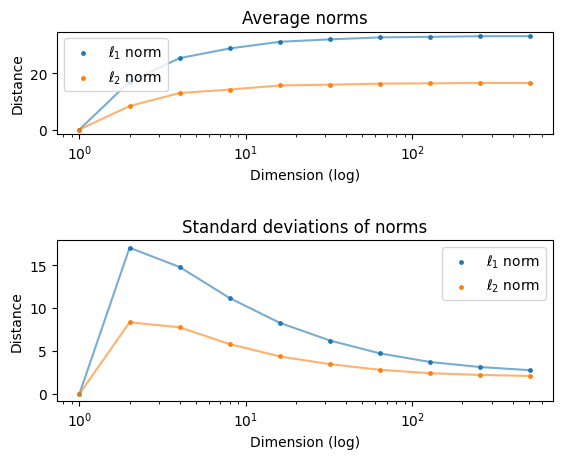
\includegraphics[width=0.6\textwidth]{../q1/figures/output.png}
        \label{fig:q1c}
    \end{figure}

    \item Since expectation is linear:
    
    \[\mathbb{E}(R) = \mathbb{E}(Z_1 + \dots + Z_d) = \sum_{i = 1}^d \mathbb{E}(Z_i) = \frac{d}{6}\]

    Since $Z_i$ are independent and identically distributed, and that variance is additive for independent random variables:

    \[\text{Var}(R) = \text{Var}(Z_1 + \dots + Z_d) = \sum_{i = 1}^d \text{Var}(Z_i) = d \cdot \frac{7}{180}\]

    \item We proceed in steps as justified in the handout. 
    \begin{enumerate}[i. ]
        \item The event ``R is at least $k$ away from its expectation'' can be written as \[E = |R - \mathbb{E}(R)| \geq k\]
        \item Using Markov's inequality, we have that \[\Pr(E) \leq \frac{\text{Var}(R)}{k^2} = \frac{d}{k^2} \cdot \frac{7}{180}\]
        \item If $k = cd$, then we have that \[\Pr(E) \leq \frac{1}{c^2 d} \cdot \frac{7}{180}\]
        With $d \to \infty$, we see that $\Pr(E) \to 0$.
    \end{enumerate}

    This supports the claim that most pairs of points are approximately the same distance. Given fixed $k$ proportional to $d$, we see that the probability of $R$ being at least $k$ away from its expectation goes to 0 as $d$ grows. That is, it is very likely that $R$ is $k$-close to its expectation as $d$ grows. More formally, given fixed $c$, we can find $d$ large enough such that for $k = cd$, we have $P(E) \leq \epsilon$, or $P(|R - \mathbb{E}(R)| < k) >  1 - \epsilon$.
\end{enumerate}


\end{document}